\section{Methods}

In this section, we give an overview of the methods we use in our analysis, namely, the backbones and the backbone distance, and the parameters we use in applying spectral clustering. We note that even though node lives in \defref{nodelife} were defined from continuous functions, we can easily apply the computation to discrete data. See \cite{BeltonExtremal22} for more details.

\subsection{Backbone Distance}

From~\figref{time-series-and-dags} and \figref{backbones}, one can see that each time series can be translated
into an ordered linear sequence of alternating minima and maxima. These linear
sequences greatly simplify the comparison between datasets. Our primary task in this section is to perform a matching operation
between the extrema of two time series. To perform the
matching, we use a modified version of the edit distance. 

\begin{figure}[htp]
     \centering
     \begin{subfigure}[b]{0.4\textwidth}
         \centering
         \includegraphics[width=\textwidth]{time-series-1.png}
         \caption{Dataset 1}
         \label{fig:timeseries1}
     \end{subfigure}
     \hfill
     \begin{subfigure}[b]{0.4\textwidth}
         \centering
         \includegraphics[width=\textwidth]{time-series-2.png}
         \caption{Dataset 2}
         \label{fig:timeseries2}
     \end{subfigure} 

        \caption{Time Series Data. We consider two datasets consisting of two functions, $\frac{1}{2}\sin(x)$ and
        $\frac{1}{2}\cos(x)$ over $[0, 2\pi]$ with some added noise. In
        \figref{timeseries1} and \figref{timeseries2}, we label the blue curve
        as ``sine-ish" and green curve as ``cosine-ish". }        
        \label{fig:time-series-and-dags}
\end{figure}

\begin{defn}[Backbones] A \emph{backbone} is a finite sequence $\x = (x_1, x_2,
    \dots , x_n)$, where each $x_i$ is a tuple~$x_i=(s_i, w_i)$ with $s_i$ a string, and $w_i \in
    \R_{\geq 0}$. The empty string is denoted by 0.
    The \emph{length} of $\x$ is denoted $\length(\x)$, and is equal to the
    number of elements in the sequence (here, $\length(\x)=n$).
    We call each $x_i$ a
    \emph{node} and we denote the first $k$ terms of $\x$ by~$\xtok{k}.$
\label{def:backbone}
\end{defn}

\begin{rem}[Constructing Backbones from Nicely Tame Functions]
    We construct a backbone from a nicely tame
    function $f \colon C \to \R$ by having a tuple for each local extrema ordered by
    domain coordinate, and weighting each of these by the node life.  This backbone for
    $f$ is denoted $B(f)$.
    See~\figref{backbones} for an example.
\end{rem}

\begin{figure}[htp]
    \centering
    \begin{subfigure}[b]{\textwidth}
        \centering
        \includegraphics[width=\textwidth]{backbone1}
        \caption{Sine Backbone 1}
        \label{fig:backbone1}
    \end{subfigure} \\
    \begin{subfigure}[b]{\textwidth}
        \centering
        \includegraphics[width=\textwidth]{backbone2}
        \caption{Sine Backbone 2}
        \label{fig:backbone2}
    \end{subfigure}
    \caption{Extracting Backbones from the two datasets.
        \figref{backbone1} illustrates the backbone where each node corresponds
        to local extrema of the sine labeled curve from Dataset 1 (see
        \figref{timeseries1}). Mathematically, this backbone is the sequence
        $(\min, 0.25)$, $(\max, 0.5)$, $(\min, 0.5)$, $(\max, 0.016)$, $(\min, 0.016)$,
        $(\max, 0.25)$.  \figref{backbone2} illustrates the backbone where each
        node corresponds to local extrema of the sine labeled curve from Dataset 2
         (see \figref{timeseries2}). Mathematically, this backbone is
        the sequence $(\min, 0.25)$, $(\max, 0.042)$, $(\min, 0.042)$, $(\max, 0.5)$,
        $(\min, 0.5)$, $(\max, 0.25)$. }
        \label{fig:backbones}
\end{figure}

Next we discuss alignments and how to compute a distance between two backbones using an optimal alignment.

\begin{defn}[Alignment]\label{def:alignment}
    %
    Let $\x = (x_1,x_2,\dots, x_m)$ and $\y = (y_1,y_2,\dots, y_n)$ be
    backbones.
    %
    Let $[k]$ denote the first $k$ natural numbers; that is,~$[k]:=\{ 1, 2, \dots, k\} \subset \N$.
    %
    An \emph{alignment} is a totally ordered correspondence between $\tilde{\x}$ and
    $\tilde{\y}$ that does not repeat elements of~$\x$ or $\y$ and respects the
    labels (or strings) of the backbones. We say that the
    number of pairs in the correspondence is the \emph{length} of the alignment.
    In particular, we represent an alignment of length $k$ between $\x$ and
    $\y$ as a  function $\alpha: [k] \to \tilde{\x} \times \tilde{\y}$,
    where $\alpha(i)$ can be written as two coordinate
    functions~$\alpha(i):= (\alpha_{\x}(i), \alpha_{\y}(i))$, such that
    %
    \begin{enumerate}
        \item \textbf{No Null Alignments.} The pair $(\zero,\zero)$ is not in the image of
            $\alpha$, which we denote by $\im(\alpha)$. \label{property:nullalignments}
        \item \textbf{Preserves Order of Backbones.} The coordinate functions $\alpha_\x: [k] \to \tilde{\x}$, $\alpha_\y:
            [k]\rightarrow \tilde{\y}$ are \emph{partially monotone}. The
            function $\alpha_\x$ is partially monotone if and only if for every
            $i,j \in [k]$ such that~$\alpha_\x(i)\neq \zero$ and $\alpha_\x(j) \neq
            \zero$, we have
            %
            $$
                \iota_\x(\alpha_\x(i)) < \iota_\x(\alpha_\x(j))
                \text{ if and only if } i < j.
            $$
            %
            An analogous definition applies to $\alpha_\y$. \label{property:preservesbackbones}
        \item \textbf{No Misalignments.}
            For each $\left((s_x,w_x),(s_y,w_y)\right) \in \im(\alpha)$,
            we either have equality in strings \mbox{$s_x = s_y$}, or one of $(s_x, w_x)$, $(s_y, w_y)$ is equal to $\zero$.  
            \label{property:nomisalignments}

        \item \textbf{Restriction to Matching.} Each element of $\x$ and $\y$ appears in the image of $\alpha_{\x}$ and $\alpha_{\y}$ exactly once. That is, for each $x_i \in \x$, there exists exactly one $j \in [k]$ for which $\alpha_{\x}(j)=x_i$. The analogous statement holds for each $y_i \in \y$. \label{property:restrictiontomatching}
    \end{enumerate}
    %
    If $\alpha(i)=(\alpha_{\x}(i), \zero)$, we say that $\alpha_{\x}(i)$ is aligned
    with an \emph{insertion}; similarly for $\alpha(i)=(\zero,\alpha_{\y}(i))$.    %
\end{defn}

 Notice that the insertions occur at the small noisy extrema in
each of the time series.

\begin{figure}[htp]
    \centering
    \begin{subfigure}[b]{\textwidth}
        \centering
        \includegraphics[width=\textwidth]{alignment1}
        \caption{Alignment 1}
        \label{fig:alignment1}
    \end{subfigure} \\
    \begin{subfigure}[b]{\textwidth}
        \centering
        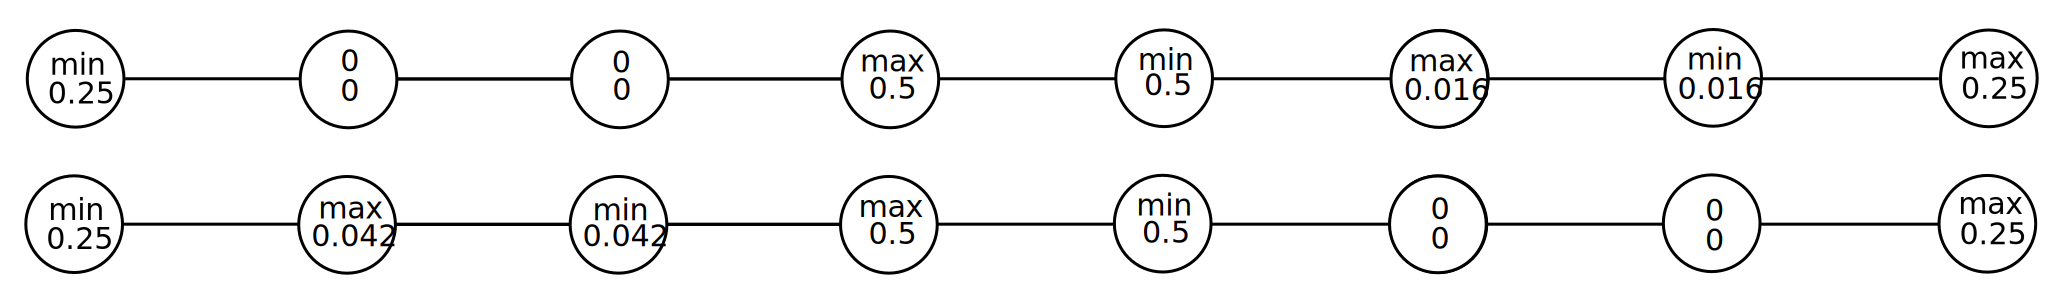
\includegraphics[width=\textwidth]{alignment2}
        \caption{Alignment 2}
        \label{fig:alignment2}
    \end{subfigure}
    %
    \caption{Two Possible Alignments of Sine Backbones. We consider the
        backbones shown in \figref{backbones}. Call these $\x$ and $\y$
        respectively. \figref{alignment1} gives an alignment, $\alpha_1: \{1, 2,
        \dots, 6\} \rightarrow \tilde{\x} \times \tilde{\y}$ of the two
        backbones where $\alpha_1(i) = (x_i, y_i)$. \figref{alignment2} gives an
        alignment $\alpha_2: \{1, 2, \dots, 8\}\rightarrow \tilde{\x} \times
        \tilde{\y}$ where $\alpha_2(1) = (x_1, y_1),$ $\alpha_2(2) = (\zero, y_2),$
        $\alpha_2(3) = (\zero, y_3),$ $\alpha_2(4) = (x_2, y_4),$
        $\alpha_2(5)=(x_3, y_5),$  $\alpha_2(6) = (x_4, \zero),$ $\alpha_2(7) =
        (x_5, \zero),$ and $\alpha_2(8) = (x_6, y_6)$.} \label{fig:alignments}
\end{figure}

\begin{defn}[Cost of Alignment]\label{def:cost}
    Let $\x$ and $\y$ be backbones and $\alpha:[k] \rightarrow \tilde{\x} \times \tilde{\y}$ be an
    alignment of length $k$. The \textit{cost} of $\alpha$ is defined as
    $$
        \cost(\alpha) := \sum_{(x,y) \in \im(\alpha)}
        |w_x-w_y|,
    $$
    where $x=(s_x,w_x)$ and $y=(s_y,w_y)$.
  \end{defn}

Referring again to~\figref{alignments}, we compute that the alignment
in~\figref{alignment2} has a lower cost, 0.116, than that
in~\figref{alignment1}, 0.932.

We define the distance between two backbones~$\x$ and~$\y$ using an
optimal alignment. 

\begin{defn}[Backbone Distance]\label{def:backbone-dist}
    %
    The \emph{backbone distance} between backbones $\x$ and $\y$ is defined
    as
    \begin{equation}%\label{backbone-dist}
    d_{\B}(\x, \y) = \inf_{\alpha}\cost(\alpha)
    \end{equation}
    where $\alpha$ ranges over all alignments between $\x$ and $\y$.
\end{defn}

The backbone distance finds the best alignment between $\x$ and $\y$, then
defines the distance to be the $L_1$-norm between a vector consisting of the
node weights in $\tilde{\x}$ and a vector consisting of the matching node weights
in $\tilde{\y}$. The backbone distance is shown to be a metric and stable in \cite{BeltonExtremal22} 
where stable means that small perturbations in the functions results in small changes in the backbone distance. 

\subsection{Spectral Clustering}
Spectral clustering is a common clustering technique on graphs that constructs clusters based on parts of the graph that are highly connected. 
See \cite{LuxburgA07} for a good overview on spectral clustering. We use the backbone distance for spectral clustering due to its properties of preserving order of local extrema, robustness to noise, and how it captures shapes of curves. Like many clustering techniques, spectral clustering involves choosing parameters. We describe how we choose those parameters here. 

\begin{itemize}
\item Similarity Matrix: To convert the backbone distance matrix to a similarity matrix, we apply the Gaussian similarity function: $s(x_i, x_j) = \text{exp}(-d_\mathcal{B}(x_i, x_j)^2/(2\sigma^2))$ where the parameter $\sigma$ controls the width of the neighborhoods. Since we are working with 10 nearest neighbors, we choose $\sigma = 0.6$ which is the average distance between a time series and its tenth nearest neighbor. 

\item Similarity Graph: We construct a similarity graph by constructing a nearest neighbors graph. We picked the number of nearest neighbors to be 10 because we want our graph to have one connected component and not super close to a complete graph. Through inspection, 10 seemed to be a good value to accomplish this. We weight the $k$-nearest neighbor graph using the similarity value computed from the Gaussian similarity of the backbone distance. Furthermore we made the similarity matrix of the similarity graph symmetric by making sure that if we have a nonzero entry at $(i,j)$, then entry $(j,i)$ had the same nonzero value.

\item Number of Clusters: We computed the graph Laplacian of the similarity matrix and then plotted the eigenvalues (see \figref{eigenvalues}) to decide the number of clusters. The plot did not give us a clear idea on the number of clusters so we made a somewhat arbitrary decision of 24. We picked 24 since it is a little larger than the number of S. Cerevisiae genes we are studying. 
\end{itemize}

\begin{figure}[htp]
    \centering
    {\includegraphics[width=.5\textwidth]{images/eigenvalues.png}} \\
    \caption{Eigenvalues in ascending order of the graph Laplacian. We see there is not a clear indicator on the number of clusters.}
    \label{fig:eigenvalues}
\end{figure}

